Express.js es un `marco de aplicación web NodeJS minimalista y flexible' \cite{express}. Es una capa delgada de características, fundamental para cualquier aplicación web, agrega tres características poderosas: enrutamiento, mejores manejadores de solicitudes y vistas.

\subsubsection{Enrutamiento}
Enrutamiento se refiere al mecanismo para servir al cliente el contenido que ha solicitado. Para las aplicaciones cliente/servidor basadas en web, el cliente especifica el contenido deseado en la URL (ruta y cadena de consulta).\\[0.8cm]
Cuando una aplicación Express.js se está ejecutando, escucha las solicitudes. Cada solicitud entrante se procesa de acuerdo con una cadena definida de middlewares y rutas que comienzan de arriba a abajo. Este aspecto es importante porque le permite controlar el flujo de ejecución \cite{azat}.
\vspace{0.8cm}

\begin{figure}[H]
  \centering
  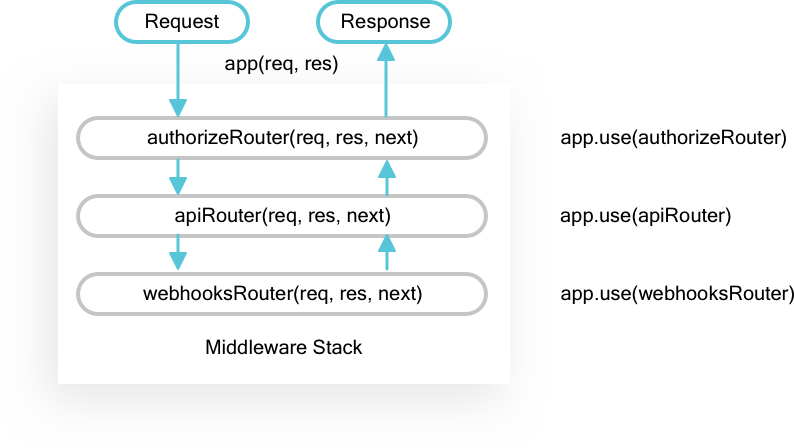
\includegraphics[width=0.8\textwidth]{express-router}
  \caption{Cada función de middleware en la pila se ejecuta antes que las que están debajo de ella.}
\end{figure}

\newpage
\lstinputlisting[style=ES6, caption=Fragmento de la configuración de enrutamiento del sistema]{code/express-router.js}